\documentclass[conference]{IEEEtran}
\IEEEoverridecommandlockouts
\usepackage{cite}
\usepackage{amsmath,amssymb,amsfonts}
\usepackage{graphicx}
\usepackage{textcomp}
\usepackage{xcolor}
\usepackage{booktabs}
\usepackage{tikz}
\usetikzlibrary{positioning}

\begin{document}

\title{Real-Time Sign Language to Speech/Text Translation Using MediaPipe Hand Landmarks and a Random Forest Classifier}

% TODO: replace the department, university and city placeholders below.
\author{\IEEEauthorblockN{Harshil Shah}
\IEEEauthorblockA{\textit{Department of [Your Department]} \\
\textit{[Your University]}\\
\textnormal{[City, Country]} \\
KUID: KU2507U0832}
\and
\IEEEauthorblockN{Dhruvil Patel}
\IEEEauthorblockA{\textit{Department of [Your Department]} \\
\textit{[Your University]}\\
\textnormal{[City, Country]} \\
KUID: 2000015222}
}

\maketitle

\begin{abstract}
Communication between deaf or hard-of-hearing people and people who do not know sign language remains a daily barrier. This paper presents a low-cost, real-time prototype that recognizes static hand gestures from an ordinary webcam and converts them into on-screen text and synthesized speech. The system uses MediaPipe Hands to extract 21 three-dimensional hand landmarks from each video frame, normalizes them into a position- and scale-invariant 63-value feature vector, and classifies the vector with a Random Forest. A confidence threshold and majority voting over recent frames stabilize the live output before a text-to-speech engine speaks the recognized word. We collected 1,981 labeled samples for six gestures from one user in one environment. On a stratified 20\% held-out split of 397 samples the classifier reached 100\% accuracy, and the live demonstration recognized the tested gestures correctly. Because the split contains consecutive frames from a single user and setting, this figure overestimates real-world performance, and we discuss this limitation explicitly. The prototype shows that landmark-based classification is a practical, affordable foundation for assistive gesture-to-speech tools.
\end{abstract}

\begin{IEEEkeywords}
sign language, hand gesture recognition, MediaPipe, computer vision, Random Forest, text-to-speech, assistive technology
\end{IEEEkeywords}

\section{Introduction}
Sign languages are the primary means of communication for many deaf and hard-of-hearing people, yet most hearing people do not know them. In everyday situations such as a shop, a clinic or a government office, this gap forces reliance on writing, gestures or an interpreter who may not be available. Technology that translates signs into text and speech can reduce this dependence and improve accessibility.

Earlier vision-based approaches often needed specialized gloves, depth sensors or large neural networks trained on extensive video datasets. These requirements make them expensive, difficult to deploy on ordinary laptops and hard to reproduce in a student project. Recent hand-tracking frameworks changed this: MediaPipe Hands estimates hand pose in real time from a single RGB camera \cite{zhang2020}, which reduces the recognition problem from raw pixels to a small vector of joint coordinates.

This work builds a complete gesture-to-speech pipeline on that idea. Its goals are to (1) recognize a small set of static hand gestures in real time using only a webcam, (2) display the result as text and speak it aloud, (3) use only free, open-source tools, and (4) evaluate the system honestly and state what the results do and do not show. The contribution is not a new recognition algorithm but an end-to-end, reproducible prototype with a documented evaluation and a candid analysis of its limitations.

\section{Related Work}
\textbf{Sign language recognition.} Research on automatic sign language recognition spans isolated-sign classification, continuous recognition and translation. Early statistical systems modeled continuous signing with hidden Markov models, and later work moved to convolutional and recurrent networks that learn directly from video \cite{koller2015,pigou2015}. Sign language translation, which generates spoken-language sentences from signing, has been studied with sequence-to-sequence neural models \cite{camgoz2018}, and a recent survey reviews deep learning methods and datasets \cite{rastgoo2021}. These systems handle richer vocabularies and motion but usually need large annotated video corpora and substantial compute.

\textbf{Hand tracking.} MediaPipe Hands \cite{zhang2020} is a two-stage on-device pipeline: a palm detector locates the hand, and a landmark model regresses 21 hand landmarks with relative depth. The detector runs only when needed, and later frames reuse the previous landmarks, which keeps the pipeline fast enough for mobile devices. It is part of the broader MediaPipe framework for perception pipelines \cite{lugaresi2019}. The tracker outputs geometry only and does not assign meaning to a gesture, so a separate classifier is required.

\textbf{Landmark-based classification.} Using landmarks as features lets a lightweight classical model replace a deep network. Random Forests \cite{breiman2001} train in seconds on small datasets, need no feature scaling and no GPU, which suits this setting. Our system follows this route and trades vocabulary size and motion handling for simplicity, speed and reproducibility.

\section{Methodology}
\subsection{System Overview}
The system is a pipeline of camera input, hand detection, landmark extraction, classification, temporal smoothing, and text and speech output (Fig.~\ref{fig:pipeline}). Three scripts implement data collection, training and live recognition.

\begin{figure}[t]
\centering
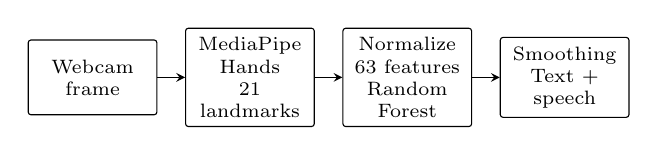
\begin{tikzpicture}[node distance=0.35cm, >=stealth,
  box/.style={draw, rounded corners=1pt, minimum height=0.95cm, text width=1.4cm, align=center, font=\scriptsize}]
\node[box] (a) {Webcam frame};
\node[box, right=of a] (b) {MediaPipe Hands\\21 landmarks};
\node[box, right=of b] (c) {Normalize\\63 features\\Random Forest};
\node[box, right=of c] (d) {Smoothing\\Text + speech};
\draw[->] (a)--(b);
\draw[->] (b)--(c);
\draw[->] (c)--(d);
\end{tikzpicture}
\caption{Overview of the gesture-to-speech pipeline.}
\label{fig:pipeline}
\end{figure}

\subsection{Gesture Set and Data Collection}
We selected six static gestures: HELLO, YES, NO, THANK\_YOU, OK and STOP. They are simple one-hand shapes that look clearly different from one another, for example an open palm (HELLO), a thumb-and-little-finger ``Y'' shape (YES), a thumbs-up (THANK\_YOU), a thumb-and-index circle (OK) and a flat upright palm (STOP). These are demonstration gestures, not official signs of American or Indian Sign Language. Real signs such as ``thank you'' involve motion, which a single-frame classifier cannot represent.

Samples were recorded with a laptop webcam. For each label the operator held the gesture in front of the camera and recorded while slightly varying hand distance and tilt. Every frame with a detected hand produced one labeled sample. Frames were mirrored horizontally in both collection and recognition. All samples were recorded with one hand, by one person, in one room under the same lighting. Table~\ref{tab:data} lists the collected samples.

\begin{table}[t]
\caption{Labeled Samples per Gesture}
\label{tab:data}
\centering
\begin{tabular}{lr}
\toprule
Gesture & Samples \\
\midrule
HELLO & 346 \\
STOP & 345 \\
NO & 336 \\
THANK\_YOU & 324 \\
YES & 317 \\
OK & 313 \\
\midrule
Total & 1,981 \\
\bottomrule
\end{tabular}
\end{table}

\subsection{Landmark Extraction and Normalization}
MediaPipe Hands was configured to track one hand with a minimum detection confidence of 0.7. For each frame it returns 21 landmarks $\mathbf{p}_i\in\mathbb{R}^3$, with $i=0$ the wrist. Raw coordinates depend on where the hand is in the image and how close it is to the camera, so each sample is normalized by subtracting the wrist and dividing by the largest absolute coordinate:
\begin{equation}
\mathbf{v}_i=\mathbf{p}_i-\mathbf{p}_0,\qquad m=\max_{i,c}\left|v_{i,c}\right|,
\end{equation}
\begin{equation}
\mathbf{f}=\frac{1}{m}\left(\mathbf{v}_0,\mathbf{v}_1,\dots,\mathbf{v}_{20}\right)\in\mathbb{R}^{63},
\end{equation}
where $c$ indexes the coordinates $x$, $y$ and $z$. The result is a 63-value vector that describes hand shape rather than position or apparent size.

\subsection{Classification}
We trained a Random Forest with 200 trees using scikit-learn \cite{pedregosa2011}. The data was split 80/20 with stratification by gesture and a fixed seed of 42. The classifier outputs a probability per gesture, which the live system uses as a confidence score.

\subsection{Real-Time Inference, Smoothing and Speech}
Per-frame predictions are noisy while the hand moves into position, so the live system adds three safeguards: (i) a prediction is accepted only if its probability exceeds 0.7; (ii) the last 10 accepted predictions are kept in a buffer, and a gesture is shown only when its label appears at least 8 times; (iii) the buffer is cleared when no hand is detected. A confirmed label is displayed on the video window and spoken with the offline pyttsx3 library, only if it differs from the last spoken label and at least two seconds have passed. Speech runs in a separate thread so the video loop does not freeze.

\section{Implementation}
The prototype is written in Python 3.12 and uses OpenCV \cite{bradski2000} for capture and display, MediaPipe 0.10.14 for hand tracking, scikit-learn 1.9.1 for the classifier, pandas for data handling and pyttsx3 for speech. It runs on a consumer Windows laptop with its built-in webcam and no GPU. The stored dataset contains landmark coordinates and labels only; no images or video are saved. All components are free and open source, and the complete code is available in the project repository.

\section{Results and Discussion}
\subsection{Offline Evaluation}
The held-out test set contains 397 samples (a stratified 20\% of the data). The classifier achieved 100\% accuracy, with precision, recall and F1-score of 1.00 for every gesture (Table~\ref{tab:results}). Class counts range from 313 to 346, so accuracy is not distorted by class imbalance.

\begin{table}[t]
\caption{Per-Gesture Results on the Held-Out Split}
\label{tab:results}
\centering
\begin{tabular}{lcccc}
\toprule
Gesture & Precision & Recall & F1 & Support \\
\midrule
HELLO & 1.00 & 1.00 & 1.00 & 69 \\
NO & 1.00 & 1.00 & 1.00 & 67 \\
OK & 1.00 & 1.00 & 1.00 & 63 \\
STOP & 1.00 & 1.00 & 1.00 & 69 \\
THANK\_YOU & 1.00 & 1.00 & 1.00 & 65 \\
YES & 1.00 & 1.00 & 1.00 & 64 \\
\midrule
Accuracy & & & 1.00 & 397 \\
\bottomrule
\end{tabular}
\end{table}

\subsection{Live Demonstration}
In the live demonstration the system displayed the recognized word as the matching gesture was held in front of the camera (Fig.~\ref{fig:demo}). Recognition appeared stable once a gesture was held steadily for about a second, which is the effect of the smoothing step. We did not measure latency or frame rate, so we make no quantitative speed claim beyond observing that the system ran interactively on a laptop webcam.

\begin{figure}[t]
\centering
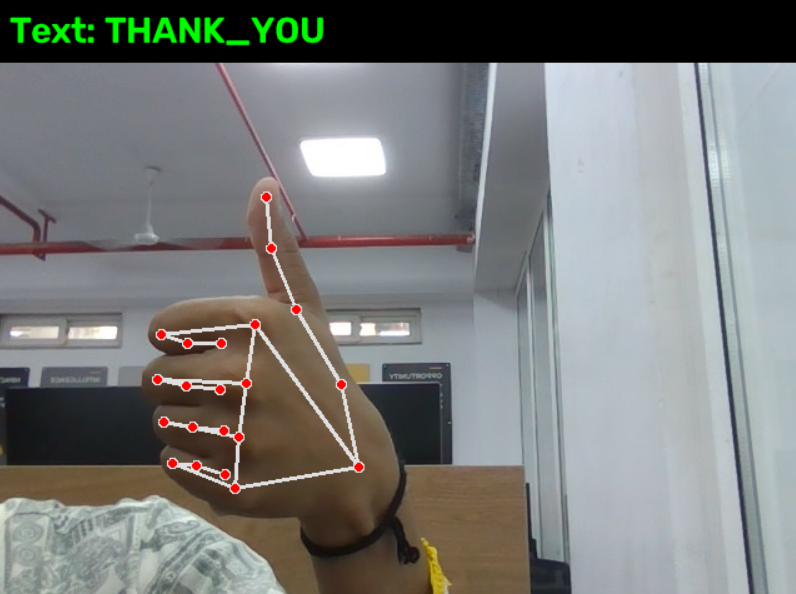
\includegraphics[width=0.31\columnwidth]{figures/demo_thankyou.png}\hspace{0.01\columnwidth}%
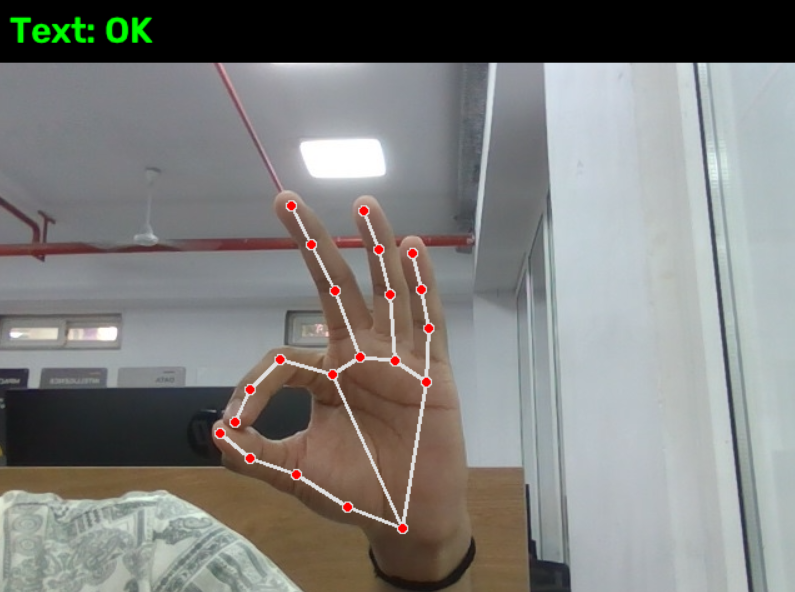
\includegraphics[width=0.31\columnwidth]{figures/demo_ok.png}\hspace{0.01\columnwidth}%
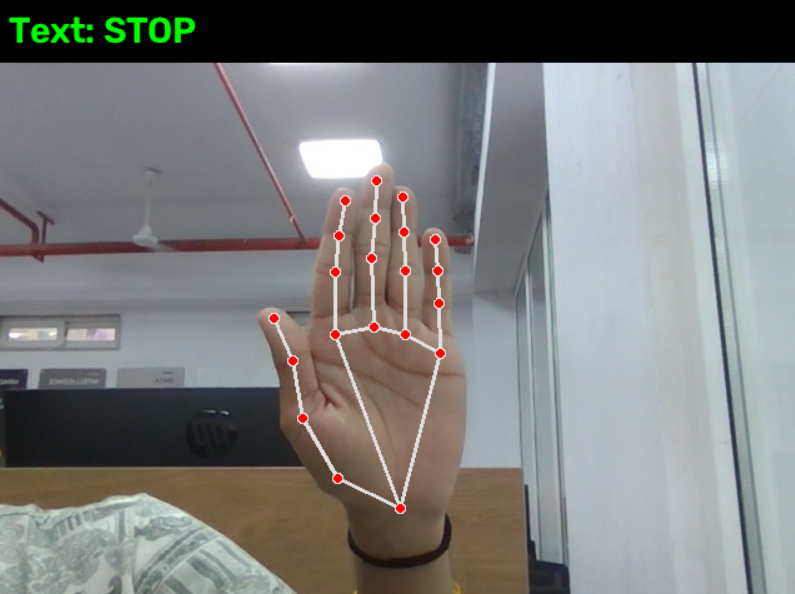
\includegraphics[width=0.31\columnwidth]{figures/demo_stop.png}
\caption{Live recognition with tracked landmarks and recognized text: THANK\_YOU, OK and STOP (left to right).}
\label{fig:demo}
\end{figure}

\subsection{Interpretation and Threats to Validity}
The perfect offline score should be read with caution. First, the data consists of consecutive video frames, so a random split places near-identical frames in both the training and test sets. Second, all data comes from one person, one hand, one room and one camera, so performance on other people, lighting and cameras is unknown. Third, the six gestures were chosen to look very different, which makes the problem easy; real vocabularies contain many similar signs. Fourth, we did not systematically test occlusion, fast movement or distance changes. A fairer evaluation would hold out entire recording sessions and participants and report accuracy under varied lighting and distance. Until then, the 100\% figure shows that the pipeline is correctly implemented and that the chosen gestures are separable in landmark space, not that the system is accurate in the real world.

\section{Limitations and Ethical Considerations}
The system recognizes static gestures only, so motion signs such as the standard ASL sign for ``thank you'' cannot be represented. The vocabulary is six demonstration gestures and does not follow a standard sign language, which also uses facial expression, posture and grammar that the system ignores. It tracks a single hand, has a small closed vocabulary, depends on MediaPipe detecting the hand, and has been evaluated on one user.

Sign languages belong to deaf communities, and any serious continuation should be designed and evaluated with deaf signers. A wrong or missing output can cause misunderstanding, so a prototype like this should not be the only means of communication in medical, legal or emergency settings. The system stores only landmark coordinates and generates speech locally, which limits personal data. Tracking quality can differ across skin tones, hand sizes and lighting, and this remains untested.

\section{Conclusion and Future Work}
We presented a real-time gesture-to-speech prototype built from a webcam, MediaPipe Hands, a Random Forest classifier and an offline text-to-speech engine. Normalizing the 21 landmarks into a 63-value, position- and scale-invariant vector allowed a lightweight classifier to separate six static gestures, and confidence thresholding with temporal smoothing produced stable live output. Future work includes multi-user and multi-session evaluation, real sign vocabularies developed with signers, sequence models such as LSTMs or Transformers for motion and sentences, two-hand and facial features, robustness to lighting, an explicit unknown-gesture class, a mobile application, and support for multiple sign languages.

\begin{thebibliography}{00}
\bibitem{zhang2020} F. Zhang et al., ``MediaPipe Hands: On-device real-time hand tracking,'' arXiv:2006.10214, 2020.
\bibitem{lugaresi2019} C. Lugaresi et al., ``MediaPipe: A framework for building perception pipelines,'' arXiv:1906.08172, 2019.
\bibitem{breiman2001} L. Breiman, ``Random forests,'' \textit{Mach. Learn.}, vol. 45, no. 1, pp. 5--32, 2001.
\bibitem{pedregosa2011} F. Pedregosa et al., ``Scikit-learn: Machine learning in Python,'' \textit{J. Mach. Learn. Res.}, vol. 12, pp. 2825--2830, 2011.
\bibitem{bradski2000} G. Bradski, ``The OpenCV library,'' \textit{Dr. Dobb's J. Softw. Tools}, 2000.
\bibitem{camgoz2018} N. C. Camgoz, S. Hadfield, O. Koller, H. Ney, and R. Bowden, ``Neural sign language translation,'' in \textit{Proc. IEEE Conf. Comput. Vis. Pattern Recognit. (CVPR)}, 2018.
\bibitem{koller2015} O. Koller, J. Forster, and H. Ney, ``Continuous sign language recognition: Towards large vocabulary statistical recognition systems handling multiple signers,'' \textit{Comput. Vis. Image Underst.}, vol. 141, pp. 108--125, 2015.
\bibitem{pigou2015} L. Pigou, S. Dieleman, P.-J. Kindermans, and B. Schrauwen, ``Sign language recognition using convolutional neural networks,'' in \textit{Computer Vision -- ECCV 2014 Workshops}. Springer, 2015.
\bibitem{rastgoo2021} R. Rastgoo, K. Kiani, and S. Escalera, ``Sign language recognition: A deep survey,'' \textit{Expert Syst. Appl.}, vol. 164, Art. no. 113794, 2021.
\end{thebibliography}

\end{document}
